\documentclass[tikz,border=10pt]{standalone}
\usetikzlibrary{arrows.meta, 
                positioning,
                calc,
                shapes.geometric
               }
\pagestyle{empty}

\begin{document}

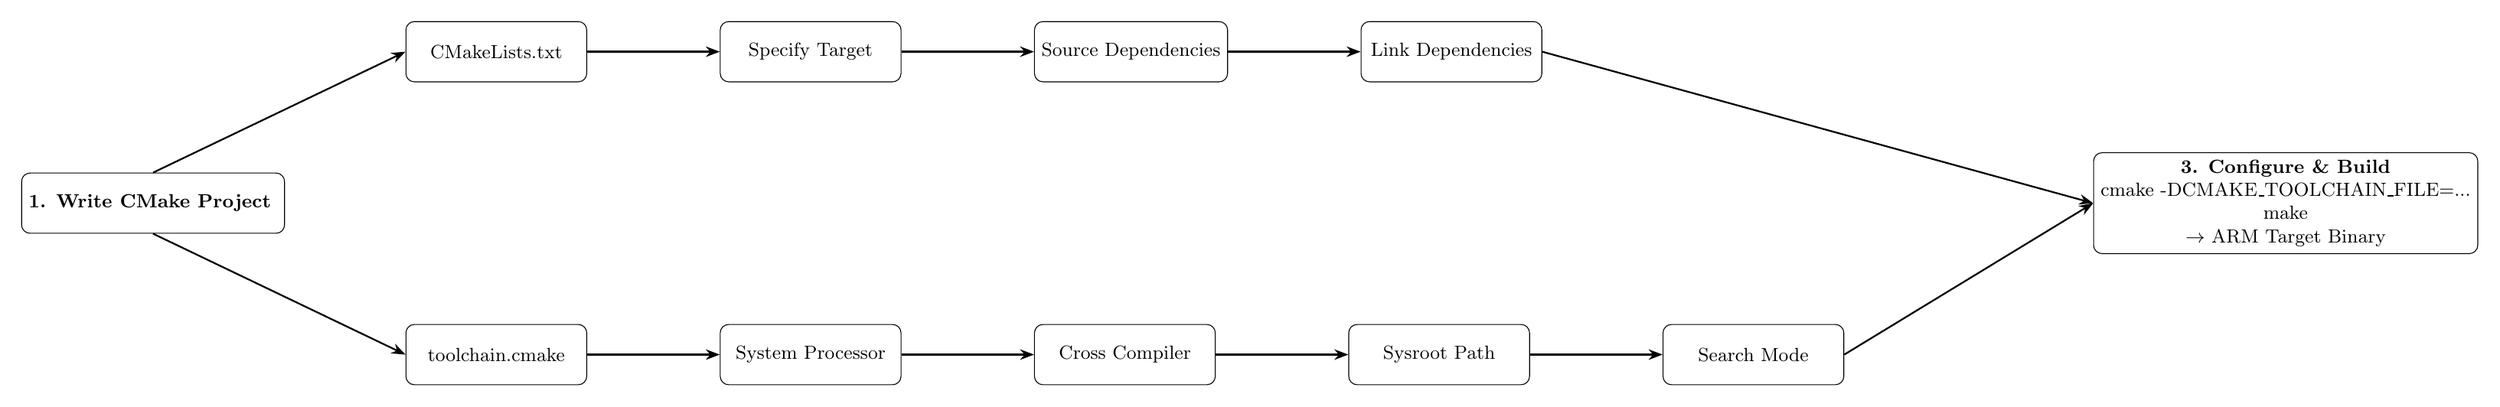
\begin{tikzpicture}[
    node distance=1.8cm and 2.2cm,
    >=Stealth,
    every node/.style={
        draw,
        rectangle,
        rounded corners,
        align=center,
        minimum width=3cm,
        minimum height=1cm,
        font=\small
    },
    arrow/.style={->, thick}
]

% --- Step 1 ---
\node (step1) {
\textbf{1. Write CMake Project}
};

% --- 2a: Build Logic (top row) ---
\node (a1) [above right=1.5cm and 2cm of step1] {CMakeLists.txt};
\node (a2) [right=of a1] {Specify Target};
\node (a3) [right=of a2] {Source Dependencies};
\node (a4) [right=of a3] {Link Dependencies};

% --- 2b: Platform Definition (bottom row, snake back) ---
\node (b1) [below right=1.5cm and 2cm of step1] {toolchain.cmake};
\node (b2) [right=of b1] {System Processor};
\node (b3) [right=of b2] {Cross Compiler};
\node (b4) [right=of b3] {Sysroot Path};
\node (b5) [right=of b4] {Search Mode};

% --- Step 3 ---
\node (step3) [right=30cm of step1] {
\textbf{3. Configure \& Build}\\
cmake -DCMAKE\_TOOLCHAIN\_FILE=...\\
make\\
$\rightarrow$ ARM Target Binary
};

% --- Arrows: split ---
\draw[arrow] (step1.north) -- (a1.west);
\draw[arrow] (step1.south) -- (b1.west);

% --- Arrows: 2a chain ---
\draw[arrow] (a1) -- (a2);
\draw[arrow] (a2) -- (a3);
\draw[arrow] (a3) -- (a4);

% --- Arrows: 2b chain (reverse direction) ---
\draw[arrow] (b1) -- (b2);
\draw[arrow] (b2) -- (b3);
\draw[arrow] (b3) -- (b4);
\draw[arrow] (b4) -- (b5);

% --- Merge into step 3 ---
\draw[arrow] (a4.east) -- (step3.west);
\draw[arrow] (b5.east) -- (step3.west);

\end{tikzpicture}

\end{document}
